% Options for packages loaded elsewhere
\PassOptionsToPackage{unicode}{hyperref}
\PassOptionsToPackage{hyphens}{url}
\PassOptionsToPackage{dvipsnames,svgnames,x11names}{xcolor}
%
\documentclass[
]{article}

\usepackage{amsmath,amssymb}
\usepackage{iftex}
\ifPDFTeX
  \usepackage[T1]{fontenc}
  \usepackage[utf8]{inputenc}
  \usepackage{textcomp} % provide euro and other symbols
\else % if luatex or xetex
  \usepackage{unicode-math}
  \defaultfontfeatures{Scale=MatchLowercase}
  \defaultfontfeatures[\rmfamily]{Ligatures=TeX,Scale=1}
\fi
\usepackage{lmodern}
\ifPDFTeX\else  
    % xetex/luatex font selection
\fi
% Use upquote if available, for straight quotes in verbatim environments
\IfFileExists{upquote.sty}{\usepackage{upquote}}{}
\IfFileExists{microtype.sty}{% use microtype if available
  \usepackage[]{microtype}
  \UseMicrotypeSet[protrusion]{basicmath} % disable protrusion for tt fonts
}{}
\makeatletter
\@ifundefined{KOMAClassName}{% if non-KOMA class
  \IfFileExists{parskip.sty}{%
    \usepackage{parskip}
  }{% else
    \setlength{\parindent}{0pt}
    \setlength{\parskip}{6pt plus 2pt minus 1pt}}
}{% if KOMA class
  \KOMAoptions{parskip=half}}
\makeatother
\usepackage{xcolor}
\usepackage[top=30mm,left=30mm,heightrounded]{geometry}
\setlength{\emergencystretch}{3em} % prevent overfull lines
\setcounter{secnumdepth}{-\maxdimen} % remove section numbering
% Make \paragraph and \subparagraph free-standing
\ifx\paragraph\undefined\else
  \let\oldparagraph\paragraph
  \renewcommand{\paragraph}[1]{\oldparagraph{#1}\mbox{}}
\fi
\ifx\subparagraph\undefined\else
  \let\oldsubparagraph\subparagraph
  \renewcommand{\subparagraph}[1]{\oldsubparagraph{#1}\mbox{}}
\fi


\providecommand{\tightlist}{%
  \setlength{\itemsep}{0pt}\setlength{\parskip}{0pt}}\usepackage{longtable,booktabs,array}
\usepackage{calc} % for calculating minipage widths
% Correct order of tables after \paragraph or \subparagraph
\usepackage{etoolbox}
\makeatletter
\patchcmd\longtable{\par}{\if@noskipsec\mbox{}\fi\par}{}{}
\makeatother
% Allow footnotes in longtable head/foot
\IfFileExists{footnotehyper.sty}{\usepackage{footnotehyper}}{\usepackage{footnote}}
\makesavenoteenv{longtable}
\usepackage{graphicx}
\makeatletter
\def\maxwidth{\ifdim\Gin@nat@width>\linewidth\linewidth\else\Gin@nat@width\fi}
\def\maxheight{\ifdim\Gin@nat@height>\textheight\textheight\else\Gin@nat@height\fi}
\makeatother
% Scale images if necessary, so that they will not overflow the page
% margins by default, and it is still possible to overwrite the defaults
% using explicit options in \includegraphics[width, height, ...]{}
\setkeys{Gin}{width=\maxwidth,height=\maxheight,keepaspectratio}
% Set default figure placement to htbp
\makeatletter
\def\fps@figure{htbp}
\makeatother
\newlength{\cslhangindent}
\setlength{\cslhangindent}{1.5em}
\newlength{\csllabelwidth}
\setlength{\csllabelwidth}{3em}
\newlength{\cslentryspacingunit} % times entry-spacing
\setlength{\cslentryspacingunit}{\parskip}
\newenvironment{CSLReferences}[2] % #1 hanging-ident, #2 entry spacing
 {% don't indent paragraphs
  \setlength{\parindent}{0pt}
  % turn on hanging indent if param 1 is 1
  \ifodd #1
  \let\oldpar\par
  \def\par{\hangindent=\cslhangindent\oldpar}
  \fi
  % set entry spacing
  \setlength{\parskip}{#2\cslentryspacingunit}
 }%
 {}
\usepackage{calc}
\newcommand{\CSLBlock}[1]{#1\hfill\break}
\newcommand{\CSLLeftMargin}[1]{\parbox[t]{\csllabelwidth}{#1}}
\newcommand{\CSLRightInline}[1]{\parbox[t]{\linewidth - \csllabelwidth}{#1}\break}
\newcommand{\CSLIndent}[1]{\hspace{\cslhangindent}#1}

\usepackage{lineno}
\linenumbers
\makeatletter
\makeatother
\makeatletter
\makeatother
\makeatletter
\@ifpackageloaded{caption}{}{\usepackage{caption}}
\AtBeginDocument{%
\ifdefined\contentsname
  \renewcommand*\contentsname{Table of contents}
\else
  \newcommand\contentsname{Table of contents}
\fi
\ifdefined\listfigurename
  \renewcommand*\listfigurename{List of Figures}
\else
  \newcommand\listfigurename{List of Figures}
\fi
\ifdefined\listtablename
  \renewcommand*\listtablename{List of Tables}
\else
  \newcommand\listtablename{List of Tables}
\fi
\ifdefined\figurename
  \renewcommand*\figurename{Figure}
\else
  \newcommand\figurename{Figure}
\fi
\ifdefined\tablename
  \renewcommand*\tablename{Table}
\else
  \newcommand\tablename{Table}
\fi
}
\@ifpackageloaded{float}{}{\usepackage{float}}
\floatstyle{ruled}
\@ifundefined{c@chapter}{\newfloat{codelisting}{h}{lop}}{\newfloat{codelisting}{h}{lop}[chapter]}
\floatname{codelisting}{Listing}
\newcommand*\listoflistings{\listof{codelisting}{List of Listings}}
\makeatother
\makeatletter
\@ifpackageloaded{caption}{}{\usepackage{caption}}
\@ifpackageloaded{subcaption}{}{\usepackage{subcaption}}
\makeatother
\makeatletter
\@ifpackageloaded{tcolorbox}{}{\usepackage[skins,breakable]{tcolorbox}}
\makeatother
\makeatletter
\@ifundefined{shadecolor}{\definecolor{shadecolor}{rgb}{.97, .97, .97}}
\makeatother
\makeatletter
\makeatother
\makeatletter
\makeatother
\ifLuaTeX
  \usepackage{selnolig}  % disable illegal ligatures
\fi
\IfFileExists{bookmark.sty}{\usepackage{bookmark}}{\usepackage{hyperref}}
\IfFileExists{xurl.sty}{\usepackage{xurl}}{} % add URL line breaks if available
\urlstyle{same} % disable monospaced font for URLs
\hypersetup{
  pdftitle={Multiproxy analysis exploring patterns of diet and disease in dental calculus and skeletal remains from a 19th century Dutch population},
  pdfauthor={Bjørn Peare Bartholdy1,; Jørgen B. Hasselstrøm2; Lambert K. Sørensen2; Maia Casna1; Menno Hoogland1; Historisch Genootschap Beemster3; Amanda G. Henry1},
  pdfkeywords={dental calculus; LC-MS/MS; alkaloids; dental pathology;
sinusitis; caffeine; tobacco},
  colorlinks=true,
  linkcolor={blue},
  filecolor={Maroon},
  citecolor={Blue},
  urlcolor={Blue},
  pdfcreator={LaTeX via pandoc}}

\title{Multiproxy analysis exploring patterns of diet and disease in
dental calculus and skeletal remains from a 19th century Dutch
population}
\author{}
\date{}

\begin{document}
\maketitle
\begin{abstract}
Dental calculus is an excellent source of information on the dietary
patterns of past populations, including consumption of plant-based
items. The detection of plant-derived residues such as alkaloids and
their metabolites in dental calculus provides direct evidence of
consumption by individuals within a population. We conducted a study on
41 individuals from Middenbeemster, a 19th century rural Dutch
archaeological site. Skeletal and dental analysis was performed to
explore potential relationships between pathological conditions/lesions
and the presence of alkaloids. We also explored other factors
potentially affecting the detection of alkaloids, including sample
weight and skeletal preservation. Dental calculus was sampled and
analysed using ultra-high-performance liquid chromatography-tandem mass
spectrometry (UHPLC-ESI-MS/MS). We were able to detect nicotine,
cotinine, caffeine, theophylline, and salicylic acid. By detecting these
compounds we are able to show the consumption of tea and coffee and
smoking of tobacco on an individual scale, which is also confirmed by
historic documentation and identification of pipe notches in the
dentition. Nicotine and/or cotinine was present in 60\% of individuals
with at least one visible pipe notch. We find some influence of skeletal
preservation on the detection of alkaloids and salicylic acid, with
higher quantities of compounds extracted from well-preserved
individuals, and also observe a relationship between weight of the
calculus sample and raw quantity of the detected compounds, and we were
able to detect alkaloids in samples as small as 2 mg. We found
correlations between chronic maxillary sinusitis and the presence of
multiple alkaloids. We show that there are many limitations that will
need to be addressed going forward with this type of analysis, and
stress the need for more systematic research on the consumption of
alkaloid-containing items and their subsequent concentration and
preservation in dental calculus, in addition to how mode of consumption
may affect concentrations on different parts of the dentition. Despite
the limitations, this preliminary study illustrates the many benefits of
using calculus to target a variety of compounds that could have been
ingested as medicine or diet, or consumed in a different manner. This
method allows us to directly address specific individuals, which can be
especially useful in individuals that are not always well-documented in
historic documentation, such as rural populations, children and women.
\end{abstract}
\ifdefined\Shaded\renewenvironment{Shaded}{\begin{tcolorbox}[breakable, interior hidden, boxrule=0pt, sharp corners, frame hidden, enhanced, borderline west={3pt}{0pt}{shadecolor}]}{\end{tcolorbox}}\fi

\textsuperscript{1} Department of Archaeological Sciences, Leiden
University\\
\textsuperscript{2} Department of Forensic Medicine, Aarhus University\\
\textsuperscript{3} Historisch Genootschap Beemster

\textsuperscript{*} Correspondence:
\href{mailto:b.p.bartholdy@arch.leidenuniv.nl}{Bjørn Peare Bartholdy
\textless{}b.p.bartholdy@arch.leidenuniv.nl\textgreater{}}

Keywords: dental calculus; LC-MS/MS; alkaloids; dental pathology;
sinusitis; caffeine; tobacco

\hypertarget{introduction}{%
\subsection{Introduction}\label{introduction}}

Dental calculus has proven to be an excellent source of a wide variety
of information about our past. The increased accessibility and
advancement of methods in aDNA, paleoproteomics, and mass spectrometry,
has expanded our ability to identify biomarkers of diet and disease on
an increasingly large scale (Gismondi et al., 2020; Velsko et al., 2017;
Warinner et al., 2014).

One such collection of biomarkers is alkaloids, a plant-derived group of
compounds. Many alkaloids have important medicinal and psychoactive
effects in humans, and their direct detection, or detection of their
metabolites, is of great interest to archaeologists. Previous studies
have successfully recovered alkaloids in archaeological contexts,
including ceramics (Smith et al., 2018), pipes (Rafferty et al., 2012),
human hair (Echeverría \& Niemeyer, 2013; Ogalde et al., 2009), and even
dental calculus employing both targeted (Eerkens et al., 2018) and
untargeted approaches (Buckley et al., 2014; Gismondi et al., 2020).
Especially nicotine, the principal alkaloid in tobacco leaves, has been
widely studied in the archaeological record due to its apparent
stability and ability to survive over long periods of time (Eerkens et
al., 2018; Rafferty et al., 2012; Tushingham et al., 2013).

Alkaloids may enter the oral cavity via two pathways: (1) direct
incorporation through oral consumption of alkaloid-containing plants,
whether deliberate or accidental; and (2) passive diffusion as alkaloids
and other compounds are transferred from plasma to saliva, and then into
the oral cavity through the salivary glands in the hours to days
following consumption (Cone \& Huestis, 2007). The relation to plasma is
why there is often a close correlation between presence (not
concentration) of drugs in oral fluid and blood (Cone \& Huestis, 2007;
Milman et al., 2011; Wille et al., 2009). The second pathway allows the
identification of parent compounds that are not consumed orally, as long
as they, or their metabolites, are excreted through saliva. .

Many of the components involved in the formation and growth of dental
calculus originate from oral fluid. Proteins, bacteria, salts and other
compounds are transferred from saliva to biofilms on the tooth surface
(Jin \& Yip, 2002; White, 1997). This may also allow various alkaloids
of dietary and medicinal origin to become incorporated in dental plaque.
Dental plaque undergoes frequent mineralisation events, ultimately
causing the entrapped alkaloids and their metabolites to become
preserved within the dental calculus. Barring intentional or accidental
removal of the calculus during life, burial, excavation, and
post-excavation cleaning, the alkaloids can then be detected by various
methods to show a record of consumption during life.

In this study we use a ultra-high-performance liquid
chromatography-tandem mass spectrometry (UHPLC-MS/MS) method that was
developed in a previous study on dental calculus from cadavers and
validated by comparing the results to compounds detected in the blood of
the same individuals (Sørensen et al., 2021). All compounds that were
detected in the blood were also detected in dental calculus, with
additional compounds present in dental calculus that were not present in
blood, suggesting that dental calculus represents a comprehensive
history of consumption over a long period of time (Sørensen et al.,
2021). We were able to detect both parent compounds and metabolites,
including caffeine, nicotine, theophylline, and cotinine, in the dental
calculus of individuals from a 19th century Dutch population from
Middenbeemster. By detecting these compounds we are able to show the
consumption of tea and coffee and smoking of tobacco on an individual
scale, which is also confirmed by historic documentation and
identification of pipe notches in the dentition.

\hypertarget{materials}{%
\subsection{Materials}\label{materials}}

The sample consists of 41 individuals from Middenbeemster, a 19th
century rural Dutch site. The village of Middenbeemster and the
surrounding Beemsterpolder was established in the beginning of the 17th
century, when the Beemster lake was drained to create more farmland,
mainly for the cultivation of cole seeds (de Vries 1978). In 1615, a
decision was made to build a church, and construction started in 1618
(Hakvoort 2013). The excavated cemetery is associated with the
Keyserkerk church, where the inhabitants of the Middenbeemster village
and the surrounding Beemsterpolder were buried between AD 1615 and 1866
(Lemmers et al., 2013). Archival documents are available for those
buried between AD 1829 and 1866, when the majority of individuals were
interred (Palmer et al., 2016). The main occupation of the inhabitants
was dairy farming, consisting largely of manual labour prior to the
industrial revolution (Aten et al., 2012; Palmer et al., 2016).

To reduce the number of potentially confounding factors to account for
in the analysis, we preferentially selected males from the middle adult
age category (35-49 years). The sample consists of 27 males, 11 probable
males, 2 probable females, and 1 female
(Figure~\ref{fig-sample-demography}). We selected males due to a higher
occurrence of pipe notches and dental calculus deposits than females
(unpublished observation).

\begin{figure}

{\centering 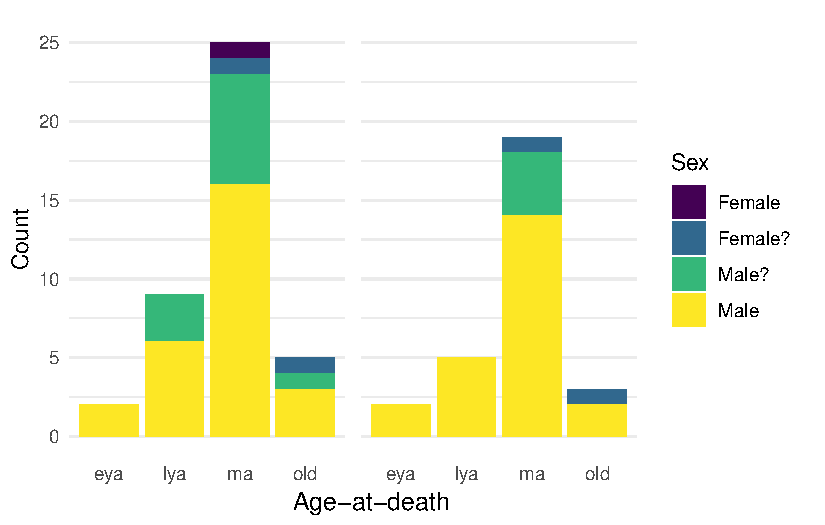
\includegraphics{paper_files/figure-pdf/fig-sample-demography-1.pdf}

}

\caption{\label{fig-sample-demography}Overview of sample demography.
Left plot is the first batch and right plot is the replication batch
with 29 of the individuals from the first batch. eya = early young adult
(18-24 years); lya = late young adult (25-34 years); ma = middle adult
(35-49 years); old = old adult (50+ years). Male? = probable male;
Female? = probable female.}

\end{figure}

\hypertarget{methods}{%
\subsection{Methods}\label{methods}}

\hypertarget{skeletal-analysis}{%
\subsubsection{Skeletal analysis}\label{skeletal-analysis}}

Demographic and pathological analyses were conducted in the Laboratory
for Human Osteoarchaeology at Leiden University. Sex was estimated using
cranial and pelvic morphological traits (Buikstra \& Ubelaker, 1994).
Age-at-death was estimated using dental wear, auricular and pubic
surface appearance, cranial suture closure, and epiphyseal fusion
(Brooks \& Suchey, 1990; Buckberry \& Chamberlain, 2002; Buikstra \&
Ubelaker, 1994; Lovejoy et al., 1985; Meindl \& Lovejoy, 1985), and
divided into the following categories: early young adult (18-24 years),
late young adult (25-34 years), middle adult ( 35-49 years), old adult
(50+ years).

\hypertarget{paleopathology}{%
\paragraph{Paleopathology}\label{paleopathology}}

Pathological conditions and lesions that occur frequently in the
population were included in the analysis. Data were dichotomised to
presence/absence to allow statistical analysis. Osteoarthritis was
considered present in cases where eburnation was visible on one or more
joint surfaces. Vertebral osteophytosis is identified by marginal
lipping and/or osteophyte formation on the margin of the superior and
inferior surfaces of the vertebral body. Cribra orbitalia was diagnosed
based on the presence of pitting on the superior surface of the orbit.
No distinction was made between active or healing lesions. Degenerative
disc disease, or spondylosis, is identified as a large diffuse
depression of the superior and/or inferior surfaces of the vertebral
body (Rogers, 2000). Schmorl's nodes are identified as any cortical
depressions on the surface of the vertebral body. Data on chronic
maxillary sinusitis from Casna et al. (2021) were included in this study
to assess the relationship between upper respiratory diseases with
environmental factors (i.e.~tobacco smoke, caffeine consumption).
Lesions associated with chronic maxillary sinusitis as defined by
Boocock et al. (1995) were recorded for each individual and classified
as ``pitting'', ``spicule-type bone formation'', ``remodeled spicules'',
or ``white pitted bone''. chronic maxillary sinusitis was scored as
absent when the sinus presented smooth surfaces with little or no
associated pitting.

\hypertarget{dental-pathology}{%
\paragraph{Dental pathology}\label{dental-pathology}}

Caries ratios were calculated by dividing the number of lesions by the
number of teeth scored, resulting in a single caries ratio per
individual. If the surface where the lesion originated is not visible,
i.e.~if the lesion covered multiple surfaces, this was scored as
``crown''. Calculus indices were calculated according to Greene and
colleagues (2005). Calculus was scored with a four-stage scoring system
(0-3) to score absent, slight, moderate, and heavy calculus deposits
(Brothwell, 1981) on the lingual, buccal (and labial), and interproximal
surfaces of each tooth. Only one score was used for the combined
interproximal surfaces, resulting in three scores per tooth (when
surfaces are intact), and four calculus indices per individual; upper
anterior, upper posterior, lower anterior, lower posterior. Each index
was calculated by dividing the sum of calculus scores for each surface
by the total number of surfaces scored in each quadrant. If a tooth
could not be scored on all three surfaces, the tooth was not included
(Greene et al., 2005). Periodontitis was scored on a visual four-stage
(0-3) scoring system according to distance from cemento-enamel junction
of each tooth to alveolar bone (Maat \& Mastwijk, 2005).

\hypertarget{calculus-sampling}{%
\subsubsection{Calculus sampling}\label{calculus-sampling}}

Where possible, we used material that had already been sampled for a
previous study to prevent unnecessary repeated sampling of individuals.
Calculus from the previous study was sampled in a dedicated ancient DNA
laboratory at the Laboratories of Molecular Anthropology and Microbiome
Research in Norman, Oklahoma, U.S.A, using established ancient DNA
protocols. More details on the methods can be found in the published
articles (Ziesemer et al., 2015, 2018). Of the 41 individuals that were
originally included in our sample, 29 were replicated in a separate
analysis only using calculus from the previous study.\\
New dental calculus samples were taken under sterile conditions in a
positive pressure laminar flow hood in a dedicated dental calculus lab
at Leiden University. The surface of the tooth was lightly brushed with
a sterile, disposable toothbrush to get rid of surface contaminants. A
sterile dental curette was then used to scrape calculus from the tooth
onto weighing paper, which was transferred to 1.5 ml Eppendorf tubes.
All calculus samples were sent to the Department of Forensic Medicine at
Aarhus University for ultra-high-performance liquid
chromatography-tandem mass spectrometry (UHPLC-MS/MS) analysis.

\hypertarget{uhplc-msms}{%
\subsubsection{UHPLC-MS/MS}\label{uhplc-msms}}

The list of targeted compounds included both naturally occurring
compounds known to have been used in the past, as well as synthetic
modern drugs that did not exist at the time (e.g.~Fentanyl, MDMA,
Amphetamine). These were part of the toxicology screening for the
original method (Sørensen et al., 2021), developed on cadavers. In our
study they serve as an authentication step, as their presence in
archaeological samples could only be the result of contamination.

Briefly, samples of dental calculus were washed three times each with
one mL of methanol (MeOH), to remove surface contaminants. The wash
solutions were collected separately. The solvent was evaporated and the
residues were dissolved in 50 µL 30\% MeOH. The washed calculus was
homogenized in presence of 0.5 M citric acid using a lysing tube with
stainless steel beads. Following one hour of incubation the dissolution
extract was cleaned by weak and strong cation-exchange. After
evaporation of the elution solvent the residue was dissolved in 50 µL
30\% MeOH. The final extracts obtained from washing and dissolution of
the dental calculus were analysed by UHPLC-MS/MS using a reversed-phase
biphenyl column for chromatography. To obtain quantitative results,
isotope dilution was applied. For more details about the method and
validation, see the original study by Sørensen and colleagues (2021).

\hypertarget{statistical-analysis}{%
\subsubsection{Statistical analysis}\label{statistical-analysis}}

All compounds and pathological conditions/lesions were converted to a
presence/absence score. Pearson product-moment correlation was applied
to the dichotomised pathological lesions (point-biserial correlation),
compound concentrations, calculus indices, and caries ratios to explore
relationships paired continuous-continuous variables and paired
continuous-binary variables. Compound concentrations were then
dichotomised to presence/absence, and the caries ratio and calculus
index for each individual were converted to an ordinal score from 0 to 4
by using quartiles. Polychoric correlation was applied to the paired
dichotomous variables and dichotomous-ordinal variables.

All statistical analysis was conducted in R version 4.3.1 (2023-06-16),
Beagle Scouts, (R Core Team, 2020). Data wrangling was conducted with
the \textbf{tidyverse} (Hadley Wickham et al., 2019) and visualisations
were created using \textbf{ggplot2} (H. Wickham, 2016). Polychoric
correlations were calculated with the \textbf{psych} package (Revelle,
2022).

\hypertarget{results}{%
\subsection{Results}\label{results}}

Multiple compounds were detected in the dental calculus samples.
Compounds detected at a lower concentration than the lower limit of
quantitation (LLOQ) were considered not present. Not all the compounds
detected in the first batch could be replicated in the second batch
(Table~\ref{tbl-compound-detect}). For a full list of targeted
compounds, see Supplementary Material.

\hypertarget{tbl-compound-detect}{}
\begin{longtable}[]{@{}lllr@{}}
\caption{\label{tbl-compound-detect}Target compound including whether it
was detected (TRUE) or not (FALSE) in each batch, as well as the lower
limit of quantitation (LLOQ) in ng. CBD = cannabidiol; CBN = cannabinol;
THC = tetrahydrocannabinol; THCA-A = tetrahydrocannabinolic acid A;
THCVA = tetrahydrocannabivarin acid.}\tabularnewline
\toprule\noalign{}
Compound & Batch 1 & Batch 2 & LLOQ \\
\midrule\noalign{}
\endfirsthead
\toprule\noalign{}
Compound & Batch 1 & Batch 2 & LLOQ \\
\midrule\noalign{}
\endhead
\bottomrule\noalign{}
\endlastfoot
CBD & TRUE & FALSE & 0.050 \\
CBN & TRUE & FALSE & 0.050 \\
Caffeine & TRUE & TRUE & 0.050 \\
Cocaine & TRUE & FALSE & 0.025 \\
Cotinine & TRUE & TRUE & 0.050 \\
Nicotine & TRUE & TRUE & 0.100 \\
Salicylic acid & TRUE & TRUE & 0.500 \\
THC & TRUE & FALSE & 0.100 \\
THCA-A & TRUE & FALSE & 0.025 \\
THCVA & TRUE & FALSE & 0.010 \\
Theophylline & TRUE & TRUE & 0.010 \\
\end{longtable}

The pattern we expect to see in authentic compounds representing
compounds trapped within the dental calculus, is a reduction in the
quantity from wash 1 to wash 3 as potential surface contaminants are
washed off, and then a spike in the final extraction when entrapped
compounds are released and detected.

Most plots show a large increase in extracted mass of a compound between
the calculus wash extracts (wash 1-3) and the dissolved calculus (calc).
Most samples containing theophylline and caffeine had the largest
quantity of the compound extracted from the first wash, then decreasing
in washes 2 and 3. There is an increase between wash 3 and the dissolved
calculus in all samples. The patterns are consistent across batches 1
and 2. Nicotine and cotinine have the same relative quantities in the
samples, i.e., the sample with the highest extracted quantity of
nicotine also had the highest extracted quantity of cotinine
Figure~\ref{fig-auth-plot-batch2}.

\begin{figure}

{\centering 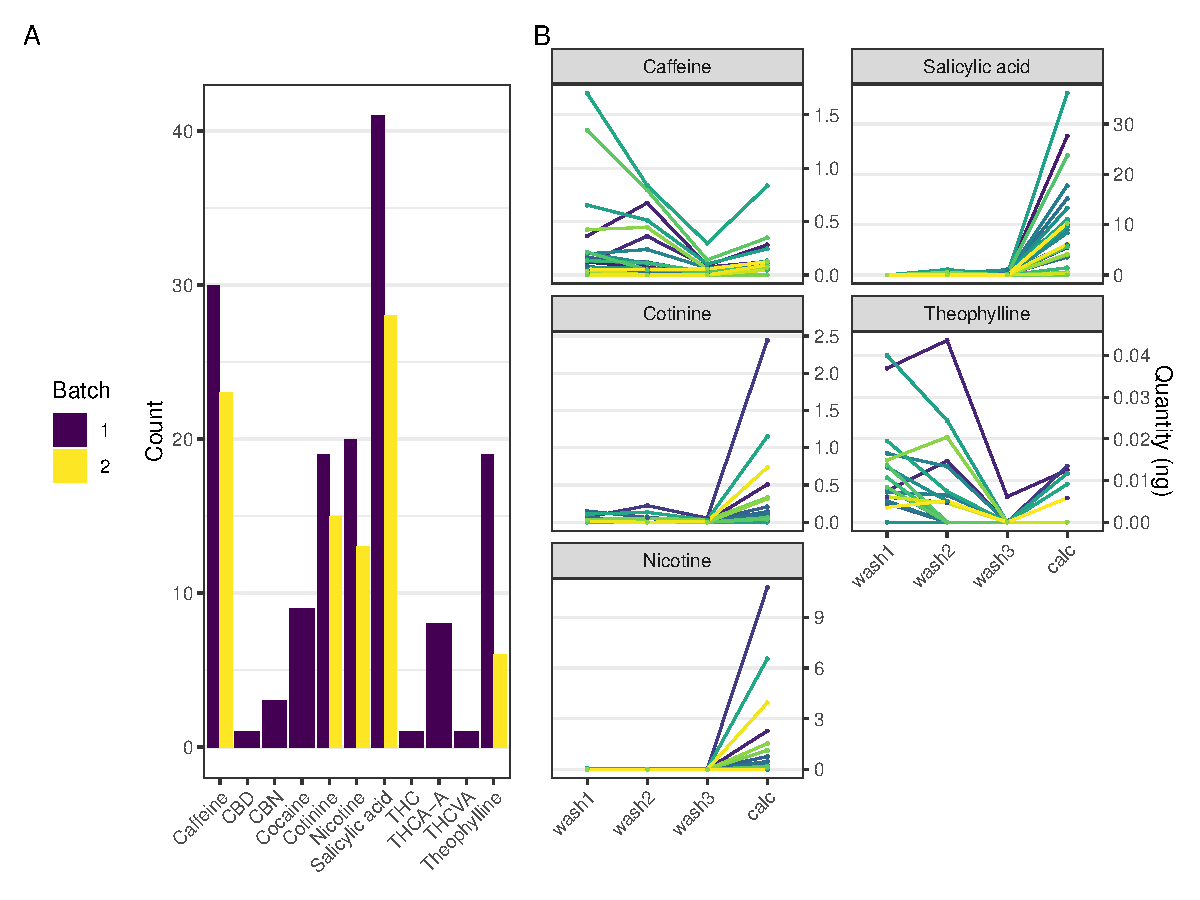
\includegraphics{paper_files/figure-pdf/fig-auth-plot-batch2-1.pdf}

}

\caption{\label{fig-auth-plot-batch2}(A) Number of samples in which each
compound was detected in the first and second batch. (B) Quantity (ng)
of each compound extracted from each sample in batch 2. The plot
displays the extracted quantity across the three washes and final
calculus extraction (calc). Each coloured line represents a different
calculus sample. CBD = cannabidiol; CBN = cannabinol; THC =
tetrahydrocannabinol; THCA-A = tetrahydrocannabinolic acid A; THCVA =
tetrahydrocannabivarin acid.}

\end{figure}

To see if preservation of the skeletal remains had any effect on the
detection of compounds, we compare extracted quantities of compounds to
the various levels of skeletal preservation. Our results from batch 2
suggest that detection of a compound may be linked to the preservation
of the skeleton, with better preservation leading to increased
extraction quantity (Figure~\ref{fig-detection-preservation}A). We also
find a weak positive correlation between the weight of the calculus
sample and the quantity of compound extracted from the calculus
(Figure~\ref{fig-detection-preservation}B).

\begin{figure}

{\centering 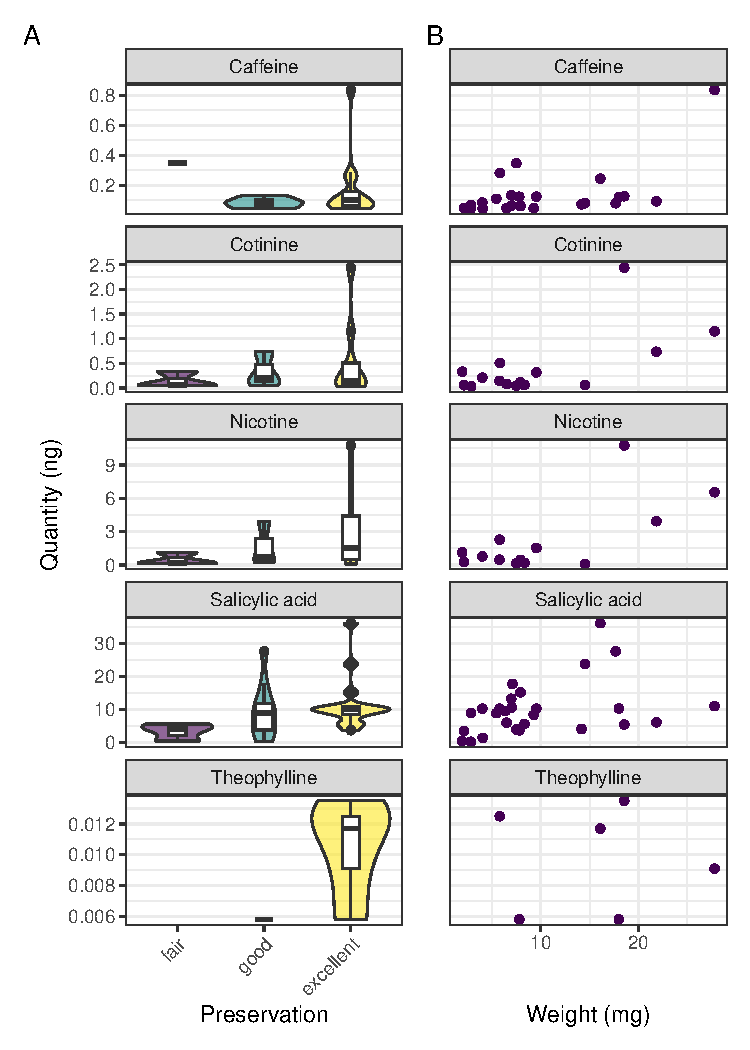
\includegraphics{paper_files/figure-pdf/fig-detection-preservation-1.pdf}

}

\caption{\label{fig-detection-preservation}(A) Violin plot with overlaid
box plots depicting the distribution of extracted quantities of each
compound from batch 2 separated by state of preservation of the
skeleton. (B) Extracted quantity (ng) of compound plotted against
weights of the calculus samples from batch 2.}

\end{figure}

The presence of pipe notch(es) in an individual and concurrent detection
of nicotine and/or cotinine is used as a crude indicator of the accuracy
of the method. Only males were used in accuracy calculations, as pipe
notches are ubiquitous in males, but not in females. In batch 2, the
method was able to detect some form of tobacco in 14 of 25 individuals
with a pipe notch (56.0\%). When also considering correct the absence of
a tobacco alkaloid together with the absence of a pipe notch, the
accuracy of the method is 59.3\%. Accuracy in the old adult age category
is 100.0\%, but with only 2 individuals.

One individual---an old adult, probable female---was positive for both
nicotine and cotinine, and had no signs of a pipe notch.

\hypertarget{correlations-between-detected-alkaloids-and-diseases}{%
\subsubsection{Correlations between detected alkaloids and
diseases}\label{correlations-between-detected-alkaloids-and-diseases}}

For further statistical analyses, only the UHPLC-MS/MS results from
batch 2 were used, as batch 1 had multiple compounds that were not
detected in batch 2 and may have been contaminated.

\hypertarget{tbl-pearson}{}
\begin{longtable}[]{@{}
  >{\raggedright\arraybackslash}p{(\columnwidth - 16\tabcolsep) * \real{0.1548}}
  >{\raggedright\arraybackslash}p{(\columnwidth - 16\tabcolsep) * \real{0.0952}}
  >{\raggedright\arraybackslash}p{(\columnwidth - 16\tabcolsep) * \real{0.1071}}
  >{\raggedright\arraybackslash}p{(\columnwidth - 16\tabcolsep) * \real{0.0833}}
  >{\raggedright\arraybackslash}p{(\columnwidth - 16\tabcolsep) * \real{0.1071}}
  >{\raggedright\arraybackslash}p{(\columnwidth - 16\tabcolsep) * \real{0.0833}}
  >{\raggedright\arraybackslash}p{(\columnwidth - 16\tabcolsep) * \real{0.1548}}
  >{\raggedright\arraybackslash}p{(\columnwidth - 16\tabcolsep) * \real{0.1071}}
  >{\raggedright\arraybackslash}p{(\columnwidth - 16\tabcolsep) * \real{0.1071}}@{}}
\caption{\label{tbl-pearson}Pearson correlation (\emph{r}) on
dichotomous skeletal lesions and compound concentrations (ng/mg) from
the second batch. Correlations between pairs of dichotomous variables
are removed due to incompatibility with a Pearson correlation. OA =
osteoarthritis; VOP = vertebral osteophytosis; SN = Schmorl's nodes; DDD
= degenerative disc disease; CO = cribra orbitalia; CMS = chronic
maxillary sinusitis; SA = salicylic acid; PN = pipe
notches.}\tabularnewline
\toprule\noalign{}
\begin{minipage}[b]{\linewidth}\raggedright
\end{minipage} & \begin{minipage}[b]{\linewidth}\raggedright
Caries
\end{minipage} & \begin{minipage}[b]{\linewidth}\raggedright
Nicotine
\end{minipage} & \begin{minipage}[b]{\linewidth}\raggedright
SA
\end{minipage} & \begin{minipage}[b]{\linewidth}\raggedright
Calculus
\end{minipage} & \begin{minipage}[b]{\linewidth}\raggedright
PN
\end{minipage} & \begin{minipage}[b]{\linewidth}\raggedright
Theophylline
\end{minipage} & \begin{minipage}[b]{\linewidth}\raggedright
Caffeine
\end{minipage} & \begin{minipage}[b]{\linewidth}\raggedright
Cotinine
\end{minipage} \\
\midrule\noalign{}
\endfirsthead
\toprule\noalign{}
\begin{minipage}[b]{\linewidth}\raggedright
\end{minipage} & \begin{minipage}[b]{\linewidth}\raggedright
Caries
\end{minipage} & \begin{minipage}[b]{\linewidth}\raggedright
Nicotine
\end{minipage} & \begin{minipage}[b]{\linewidth}\raggedright
SA
\end{minipage} & \begin{minipage}[b]{\linewidth}\raggedright
Calculus
\end{minipage} & \begin{minipage}[b]{\linewidth}\raggedright
PN
\end{minipage} & \begin{minipage}[b]{\linewidth}\raggedright
Theophylline
\end{minipage} & \begin{minipage}[b]{\linewidth}\raggedright
Caffeine
\end{minipage} & \begin{minipage}[b]{\linewidth}\raggedright
Cotinine
\end{minipage} \\
\midrule\noalign{}
\endhead
\bottomrule\noalign{}
\endlastfoot
OA & -0.12 & -0.074 & 0.21 & 0.07 & 0.14 & 0.28 & 0.00098 & -0.067 \\
VOP & -0.088 & -0.16 & 0.34 & 0.061 & 0.25 & -0.06 & 0.013 & -0.13 \\
SN & -0.24 & 0.16 & 0.095 & 0.089 & 0.17 & 0.24 & 0.16 & 0.093 \\
DDD & -0.0038 & 0.0037 & 0.19 & -0.39 & -0.077 & 0.31 & 0.06 &
-0.0086 \\
CO & 0.064 & -0.051 & 0.2 & 0.14 & -0.2 & -0.11 & 0.19 & -0.065 \\
CMS & -0.19 & 0.28 & 0.0017 & -0.27 & 0.032 & 0.19 & 0.36 & 0.22 \\
Caries & & -0.2 & -0.36 & -0.15 & -0.17 & -0.21 & -0.0045 & -0.22 \\
Nicotine & & & -0.21 & 0.01 & -0.014 & 0.43 & 0.14 & 0.98 \\
SA & & & & 0.14 & 0.37 & 0.038 & 0.17 & -0.17 \\
Calculus & & & & & 0.13 & -0.15 & -0.13 & 0.031 \\
PN & & & & & & -0.16 & 0.18 & -0.0068 \\
Theophylline & & & & & & & 0.51 & 0.36 \\
Caffeine & & & & & & & & 0.078 \\
\end{longtable}

Point-biserial correlation was conducted on paired continuous and
dichotomous variables, to see if any relationships exist between
extracted concentrations and other variables. The strongest
point-biserial (Pearson) correlation correlations were a near-perfect
positive correlation between cotinine and nicotine (0.982), and moderate
correlations between theophylline and nicotine (0.432), caffeine and
theophylline (0.507) (Table~\ref{tbl-pearson}).

Polychoric correlation was conducted on the dichotomised compounds and
pathological conditions, as well as the discretised dental diseases.
Salicylic acid was removed due to its ubiquitous presence in the sample,
and is likely to cause spurious correlations. Strong correlations were
found between cotinine and nicotine (0.847). Moderate correlations were
found between OA and DDD (0.47), VOP and periodontitis (0.487), SN and
cotinine (0.559), DDD and calculus (-0.416), CMS and caffeine (0.53),
caries and periodontitis (0.523), periodontitis and VOP (0.487),
periodontitis and age-at-death (0.407), nicotine and SN (0.53), calculus
and DDD (-0.416), age-at-death and theophylline (-0.45), theophylline
and age-at-death (-0.45), caffeine and periodontitis (0.494), cotinine
and CMS (0.427). Remaining correlations were weak or absent
(Figure~\ref{fig-polycorr}). Correlations with age will be depressed
because age was largely controlled for in the sample selection.

\begin{figure}

{\centering 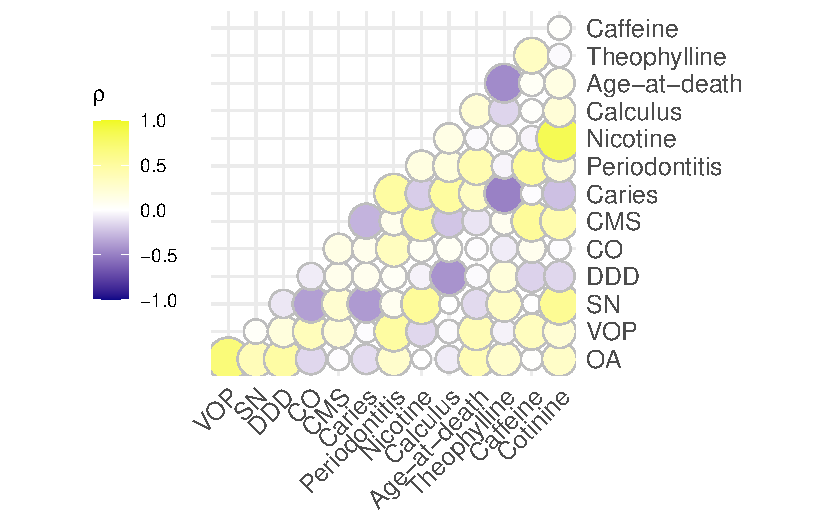
\includegraphics{paper_files/figure-pdf/fig-polycorr-1.pdf}

}

\caption{\label{fig-polycorr}Plot of the polychoric correlations
(\emph{rho}). Larger circles and increased opacity indicates a stronger
correlation coefficient. OA = osteoarthritis; VOP = vertebral
osteophytosis; SN = Schmorl's nodes; DDD = degenerative disc disease; CO
= cribra orbitalia; CMS = chronic maxillary sinusitis; SA = salicylic
acid.}

\end{figure}

\hypertarget{discussion}{%
\subsection{Discussion}\label{discussion}}

In this study we were able to extract and identify multiple alkaloids
and salicylic acid from the dental calculus of individuals from
Middenbeemster, a 19th century Dutch archaeological site. We applied
ultra-high-performance liquid chromatography-tandem mass spectrometry
(UHPLC-MS/MS), a method that was validated by co-occurrence of drugs and
metabolites in dental calculus and blood (Sørensen et al., 2021). Here
we have shown that the method can also be successfully applied to
archaeological dental calculus. We extend findings from previous studies
on alkaloids in archaeological samples by extracting multiple different
alkaloids from dental calculus, including nicotine, cotinine, caffeine,
theophylline, and salicylic acid in multiple individuals. The detection
of these compounds was solidified in a replication analysis on different
samples from the same individuals. Cocaine and multiple cannabinoids
were also detected during the first analysis, but were not replicated.
We discuss the implications of these findings in light of historical and
archaeological evidence for the consumption of these drugs.

Nicotine and its principal/main metabolite, cotinine, were strongly
positively correlated, both in concentration and presence/absence in
individuals (Table~\ref{tbl-pearson} and Figure~\ref{fig-polycorr}). The
detection of nicotine and cotinine is not surprising, as pipe-smoking in
the Beemsterpolder is well-documented in the literature (Aten et al.,
2012; Bouman, 2017), and visible on the skeletal remains as pipe notches
(Lemmers et al., 2013). There is also documented medicinal use of
nicotine in the Beemsterpolder, where a tobacco-smoke enema was used for
headaches, respiratory problems, colds, and drowsiness from around 1780
to 1830 (Aten et al., 2012). In our sample, we also detected nicotine
and cotinine (replicated) in an old adult, probable female individual.
In this particular case it is unlikely that the compounds entered the
dental calculus through pipe-smoking, as the individual had no visible
pipe notches; more likely the tobacco entered through an alternate mode
of consumption, secondhand smoke, or the aforementioned tobacco-smoke
enema.

Theophylline and caffeine were positively correlated in our samples,
though to a lesser extent than nicotine and cotinine, so we are unable
to determine if they originated from the same source
(Table~\ref{tbl-pearson} and Figure~\ref{fig-polycorr}). Caffeine and
theophylline have very similar chemical structures, so we expect they
would experience similar rates of incorporation and degradation,
allowing us to interpret the ratio and correlations between the
compounds. Caffeine is present in coffee, tea, and cocoa beans, with
concentrations slightly higher in coffee (Bispo et al., 2002; Chin et
al., 2008; Srdjenovic et al., 2008; Stavric et al., 1988). Theophylline
is present in both coffee beans and tea leaves, but in negligible
quantities (Stavric et al., 1988). It is also a primary metabolite of
caffeine produced by the liver. Given the low correlation, there are
likely multiple sources of caffeine and theophylline in the population,
with tea and coffee being the most obvious.\\
Tea consumption had become widespread in the Netherlands by 1820,
reaching all parts of society (Nierstrasz, 2015, p. 91). Historically,
we also know that both tea and coffee were consumed in the
Beemsterpolder during the 19th century. `Theegasten' (teatime) was a
special occasion occurring from 15.00-20.00 hours, where tea was served
along with the evening bread (Schuijtemaker, 2011). Many households also
owned at least one coffee pot and tea pot (Bouman, 2017). Distinguishing
between tea, coffee, and chocolate may be possible by also including
theobromine and comparing ratios of the compounds, as theobromine is
present in higher quantities in chocolate compared to caffeine and
theophylline (Alañón et al., 2016; Bispo et al., 2002; Stavric et al.,
1988). However, In addition to oral factors affecting alkaloid uptake in
dental calculus, there is some indication that theobromine does not
preserve well in the archaeological record (Velsko et al., 2017), and
frequent consumption of all three items would be difficult to parse.

Salicylic acid was found in all but one individual in our sample. It can
be extracted from the bark of willow trees, \emph{Salix alba}, and has
long been used for its pain-relieving properties (Bruinsma, 1872, p.
119). It is also present in many plant-based foods (Duthie \& Wood,
2011; Malakar et al., 2017), including potatoes, which were a staple of
the Beemsterpolder diet (Aten et al., 2012). The extracted quantity from
our samples decreased over the three washes, followed by a sharp
increase in the final calculus extraction, which is what we would expect
to see if the salicylic acid was incorporated during life
Figure~\ref{fig-auth-plot-batch2}. However, it has been shown that
salicilyc acid is a very mobile organic acid and the ubiquitous presence
may be due to environmental contamination, which would also explain the
high quantity in the washes (Badri \& Vivanco, 2009; Chen et al., 2001).
Given the multiple plausible sources of this residue, it will be
necessary to explore the extent to which salicylic acid can leach into
the dental calculus from the soil, and what the rate of degradation is
for salicylic acid when trapped in dental calculus.

Cannabinoids---specifically THC, THCA-A, THCVA, CBD, CBN---were found in
the first batch, but none were replicated in the second batch. Medicinal
use of cannabinoids has been well-established in Europe since
Medieval-times, and it was also grown in the Netherlands (Bruinsma,
1872). Administration was most common in the form of concoctions
containing various portions of the cannabis plant for ingestion; not
until the late 19th century did it become recommended to smoke it for
more immediate effects (Clarke, 2013). A Dutch medicinal use of hemp
involved an emulsion prepared from the seeds of the plants to treat pain
and various stomach ailments. Another preparation involving the roots of
the plants was used for inflammation, gout, and joint pains (Clarke,
2013). The ability to detect cannabinoids in calculus may be limited by
their reduced ability to diffuse from serum to salivary glands due to an
affinity for protein-binding, (Cone \& Huestis, 2007), meaning detection
would rely on oral consumption. Even then, the overall instability of
some cannabinoids could also affect detection (Lindholst, 2010; Sørensen
\& Hasselstrøm, 2018). However, given the lack of replication, we cannot
with security confirm that cannabis was used by the Beemster population.

Despite many of our sampled individuals having lived during the height
of the opium era in the Netherlands (Macht, 1915), none of the targeted
opioids (morphine, codeine, thebaine, papaverine, norcodeine, noscapine)
were detected. The absence of opioids could be a result of the people
ascribing more to the ``traditional'' rather than ``scientific''
medicine, although laudanum and another opium containing concoction was
part of the ``traditional'' medicine in the Netherlands (Leuw \&
Marshall, 1994), including Middenbeemster (Aten et al., 2012). It was
also generally considered a drug of the upper class (Scheltema, 1907),
and may have been more common in urban centers. The absence could also
be attributed to postmortem degradation. It has been shown that, while
abundant in opium, morphine degrades rapidly, while thebaine and
papaverine are more resistant to various ageing processes (Chovanec et
al., 2012). The latter were also absent from our samples.

The only strictly modern compound (at least in a European context)
detected in the sample was cocaine, which was detected in the first
batch of samples. Our sample is derived from an early--mid 19th century
population, and cocaine was isolated in 1860 by Albert Niemann, and
entered popular medical practice in 1884. Coca arrived in Europe as
early as 1771, but as botanical specimens rather than for consumption,
and there were also issues importing enough viable specimens of coca for
cocaine extraction (Abduca, 2019, p. 108; Mortimer, 1901, p. 179). We
considered it possible that it would be present in a sample with most
individuals originating from the early- to mid-19th century. If
corroborated, this would have been the first case of
coca-leaf-consumption in Europe. In our replication batch, we included
all of the individuals who had been cocaine-positive in the first batch.
We were unable to replicate any of the cocaine results, and we were
unable to detect the principal metabolite, benzoylecgonine, in either
batch. We suspect that the original detection of cocaine was a result of
lab contamination during analysis.

We explored the relationship between detected compounds and various
skeletal indicators, such as pathological and dental lesions,
preservation, and pipe notches. We found some evidence to suggest that
preservation of the skeleton influences the recovery of compounds from
the dental calculus, with well-preserved skeletons potentially serving
as a better target for sampling.\\
We found a positive correlation between CMS and nicotine, which may be
indicative of the impact tobacco smoking had on the respiratory health
of the Beemster inhabitants. Tobacco smoke may play a significant role
in diseases of the upper respiratory tract, including chronic maxillary
sinusities (Reh et al., 2012). Although the mechanisms by which smoking
increases the risk of infections is not fully understood, solid evidence
has been presented linking tobacco smoke to increased mucosal
permeability and impairment of mucociliary clearance (Arcavi \&
Benowitz, 2004). Such changes, together with an altered immunologic
response, are thought to predispose to the development of chronic
maxillary sinusitis (Slavin et al., 2005).\\
We also observed a moderate positive correlation between chronic
maxillary sinusitis and caffeine which contradicts previous research
linking chronic coffee consumption with a positive effect on the
respiratory system, suggesting a preventive association between caffeine
intake and pneumonia (e.g. Alfaro et al., 2018; Kondo et al., 2021).
However, while the lower respiratory tract seems to benefit from chronic
coffee consumption, it is possible that elevated caffeine intake impacts
mucosal moisture due to its dehydrating effect (Maughan \& Griffin,
2003), thereby exposing individuals to greater risk of sinus infection.

The detection of nicotine in dental calculus has previously been
presented by Eerkens and colleagues (2018) in two individuals from
pre-contact California. They also targeted caffeine, cotinine, and
theophylline in their samples, but were unable to detect any of them. It
remains to be seen whether this is due to differences in methods used,
or due to our samples being more recent. They also suggest that the
choice of tooth for sampling may impact the detection of certain
compounds, as the incorporation in dental calculus may depend on the
mode of consumption. Tobacco smokers may have more nicotine present in
calculus on incisors, whereas tobacco chewers may have more on molars
(Eerkens et al., 2018). However, sampling may not be limited to mode of
consumption. The presence of cotinine suggests that the excretion of a
compound after being metabolised in the body is also a source of
deposition, and that deposition of alkaloids in dental calculus can
occur both on the way into the body, i.e.~during consumption, and on the
way out, i.e.~disposal of waste products via saliva secretion into the
mouth. Especially mucin-rich saliva from the sublingual and
submandibular glands preferentially binds toxins (Dodds et al., 2005),
and since these glands are located closest to the lower incisors, they
may be the most effective target for these studies. This has yet to be
systematically tested in archaeological dental calculus. Because we
homogenised samples from multiple teeth of an individual, we were unable
to test the effect of oral biogeography. It is also possible that
resident microflora within biofilms contribute to alkaloid breakdown and
that the presence of caffeine and nicotine metabolites following direct
ingestion can be explained by this pathway. However, the literature on
biofilm biodegradation of alkaloids is limited, and \emph{in vitro}
studies have only found minimal contributions by certain oral bacteria
in isolation (Cogo et al., 2008; Sun et al., 2016); it is possible that
a larger role is played by oral bacteria within larger, more
metabolically active communities, e.g.~biofilms (Takahashi, 2015).

Because we targeted individuals with moderate-to-large calculus
deposits, it is likely a biased sample. The presence of calculus may
increase the risk of premature death (Yaussy \& DeWitte, 2019), and
periodontal disease (which may or may not be associated with dental
calculus build-up) is a risk-factor for respiratory diseases, if
periodontal and respiratory pathogens enter the bloodstream (Azarpazhooh
\& Leake, 2006; Scannapieco, 1999; Scannapieco \& Ho, 2001). In our
sample, the percentage of chronic maxillary sinusitis (37.0\%) is lower
than in another (more representative) male sample (44.1\%) (Casna et
al., 2021), and the caries percentage is similarly lower in our sample
(17.6\%) than a more representative sample (22.9\%) (Lemmers et al.,
2013).\\
We used the presence/absence of a pipe notch and concurrent detection of
tobacco as a crude estimate of the accuracy of the method, which we
found to be around 59.3\%. This is a very rough estimate, as the
presence of a pipe notch is likely not a perfect indicator of whether or
not someone consumed tobacco. Dental calculus is also more transient
than for example bone, as it can be mechanically removed, intentionally
or unintentionally, during life, eliminating all trace of the alkaloids
consumed prior to its removal.\\
Quantitation of the detected compounds may have limited value in
archaeological samples due to degradation, and will greatly affect our
correlations related to concentration. Following burial, compound
stability over time will play a large role, as will microbial
degradation of compounds by bacteria and fungi in soil (Liu et al.,
2015), as well as the soil environment, such as temperature, pH, and
oxygen availability (Lindholst, 2010; Mackie et al., 2017).\\
The detected quantity of a compound will also depend on the quantity in
dental calculus during life, which is largely controlled by quantity of
consumption, how often the calculus was disrupted/removed, metabolic
breakdown of the compound, and inter- and intra-individual factors
related to stages of biofilm formation, maturation, and mineralisation
(Lustmann et al., 1976; Velsko et al., 2019; Zijnge et al., 2010). In
short, this means it is not really possible to detect the absence of a
compound. The absence of a compound is not evidence of absence of
consumption. This complicates the interpretation of our results. We have
attempted to minimise errors occurring due to this limitation by
including a relatively large sample of individuals and replicating our
analysis. Although given the relatively low detection rate seen in
tobacco, this remains a major limitation, and will likely be compounded
by increasing antiquity of the samples.

Future studies should explore how sampling from various types of teeth
and their position in the mouth affects the probability of a compound
becoming entrapped in dental calculus. This may also be related to
properties within the oral cavity, as well as chemical properties of the
compounds, which facilitate or reduce the incorporation-potential, and
which incorporation pathways are more likely for a given compound.\\
We only targeted drugs that were included in the forensic toxicological
screenings, and therefore only covered a limited number of the potential
compounds that could be of interest for exploring past diets and
medicinal treatments. The list of targeted compounds can be expanded as
we discover more potential targets based on which specific
compounds/metabolites are more likely to be incorporated and preserved
in dental calculus.\\
There is an increasing interest in using oral fluid as a means of
detecting alkaloids in living individuals due to the non-invasive nature
of the testing compared to blood and urine sampling (Cone, 1993; Valen
et al., 2017). These \emph{in vivo} studies are a valuable source of
method validation and can help determine the feasibility of detecting
certain alkaloids in oral fluid and, subsequently, dental calculus.
Archaeologists, though, will likely be responsible for exploring dental
calculus specific incorporation and retention of alkaloids, as well as
their long-term preservation in the burial environment.

While a major limitation is the uncertainty surrounding whether or not a
compound is actually absent, the power of the method lies in the ability
to detect dietary and other compounds that were incorporated via
multiple consumption pathways that are not detected by other methods.
Taking tobacco consumption as an example; while pipe notches are a
useful way to identify tobacco consumption, pipe smoking was not the
only mode of tobacco consumption, with others including chewing,
drinking, cigars, and snuff (Goodman, 1994, p. 67). Pipe-smoking was
mainly practised by males (Eerkens et al., 2018; Lemmers et al., 2013),
so methods like the one presented here are suitable for exploring
tobacco consumption in an entire society, rather than a trivial subset
of past populations. Combined with other methods, it can also give us a
more complete picture of dietary patterns and medicinal/recreational
plant-use in the past by capturing multiple possible incorporation
pathways of dietary (and other) compounds.

\hypertarget{conclusions}{%
\subsection{Conclusions}\label{conclusions}}

This preliminary study outlines the benefits of using calculus to target
a variety of compounds that could have been consumed as medicine or
diet. This method allows us to directly address specific individuals,
which can be especially useful in individuals that are not always
well-documented in historic documentation, such as rural communities,
children and women. We also show that there are many limitations that
will need to be addressed going forward with this type of analysis, and
stress the need for more systematic research on the consumption of
alkaloid-containing items and their subsequent concentration and
preservation in dental calculus, in addition to how mode of consumption
may affect concentrations on different parts of the dentition. Another
limitation of dental calculus as a medium is the inter- and
intra-individual variability of its formation and the many factors that
can influence incorporation and retention of molecules and particles;
however, in the absence of hair and serum (quite uncommon in
archaeology), dental calculus represents an impressive long-term
reservoir of information regarding the consumption of various alkaloids,
whether dietary, medicinal, recreational, or otherwise.

\hypertarget{acknowledgements}{%
\subsection*{Acknowledgements}\label{acknowledgements}}
\addcontentsline{toc}{subsection}{Acknowledgements}

We wish to thank Kirsten Ziesemer for helping track down the calculus
samples from her studies. Additionally, we owe special thanks to Vincent
Falger and Kees de Groot from the Middenbeemster Historical Society for
their input on early draft manuscripts and a lovely guided tour of
Middenbeemster.

This research has received funding from the European Research Council
under the European Union's Horizon 2020 research and innovation program,
grant agreement number STG--677576 (``HARVEST'').

\hypertarget{data-availability-statement}{%
\subsection*{Data Availability
Statement}\label{data-availability-statement}}
\addcontentsline{toc}{subsection}{Data Availability Statement}

All raw data is available on Zenodo
(\url{https://doi.org/10.5281/zenodo.8061483}). Analysis scripts, and
the source code for the manuscript and supplementary materials are
available as a research compendium
(\url{https://doi.org/10.5281/zenodo.7649825}) using the structure
recommended by the \textbf{rrtools} R package (Marwick, 2019).

\hypertarget{conflict-of-interest-disclosure}{%
\subsection*{Conflict of interest
disclosure}\label{conflict-of-interest-disclosure}}
\addcontentsline{toc}{subsection}{Conflict of interest disclosure}

The authors have no conflicts to declare.

\hypertarget{references}{%
\subsection*{References}\label{references}}
\addcontentsline{toc}{subsection}{References}

\hypertarget{refs}{}
\begin{CSLReferences}{1}{0}
\leavevmode\vadjust pre{\hypertarget{ref-abucaCocaTrade2019}{}}%
Abduca, R. (2019). Coca leaf transfers to {Europe}. {Effects} on the
consumption of coca in {North-western Argentina}. In M. Kaller \& F.
Jacob (Eds.), \emph{Transatlantic {Trade} and {Global Cultural Transfers
Since} 1492: {More} than {Commodities}}. {Routledge}.
\url{https://books.google.com?id=13imDwAAQBAJ}

\leavevmode\vadjust pre{\hypertarget{ref-alanonAssessmentFlavanol2016}{}}%
Alañón, M. E., Castle, S. M., Siswanto, P. J., Cifuentes-Gómez, T., \&
Spencer, J. P. E. (2016). Assessment of flavanol stereoisomers and
caffeine and theobromine content in commercial chocolates. \emph{Food
Chemistry}, \emph{208}, 177--184.
\url{https://doi.org/10.1016/j.foodchem.2016.03.116}

\leavevmode\vadjust pre{\hypertarget{ref-alfaroChronicCoffee2018}{}}%
Alfaro, T. M., Monteiro, R. A., Cunha, R. A., \& Cordeiro, C. R. (2018).
Chronic coffee consumption and respiratory disease: {A} systematic
review. \emph{The Clinical Respiratory Journal}, \emph{12}(3),
1283--1294. \url{https://doi.org/10.1111/crj.12662}

\leavevmode\vadjust pre{\hypertarget{ref-arcaviCigaretteSmoking2004}{}}%
Arcavi, L., \& Benowitz, N. L. (2004). Cigarette {Smoking} and
{Infection}. \emph{Archives of Internal Medicine}, \emph{164}(20),
2206--2216. \url{https://doi.org/10.1001/archinte.164.20.2206}

\leavevmode\vadjust pre{\hypertarget{ref-aten400Jaar2012}{}}%
Aten, D., Bossaers, K. W. J. M., \& Misset, C. (2012). \emph{400 jaar
Beemster: 1612-2012}. {Stichting Uitgeverij Noord-Holland}.

\leavevmode\vadjust pre{\hypertarget{ref-azarpazhoohSystematicReview2006}{}}%
Azarpazhooh, A., \& Leake, J. L. (2006). Systematic {Review} of the
{Association Between Respiratory Diseases} and {Oral Health}.
\emph{Journal of Periodontology}, \emph{77}(9), 1465--1482.
\url{https://doi.org/10.1902/jop.2006.060010}

\leavevmode\vadjust pre{\hypertarget{ref-badriRegulationFunction2009}{}}%
Badri, D. V., \& Vivanco, J. M. (2009). Regulation and function of root
exudates. \emph{Plant, Cell \& Environment}, \emph{32}(6), 666--681.
\url{https://doi.org/10.1111/j.1365-3040.2009.01926.x}

\leavevmode\vadjust pre{\hypertarget{ref-bispoSimultaneousDetermination2002}{}}%
Bispo, M. S., Veloso, M. C. C., Pinheiro, H. L. C., De Oliveira, R. F.
S., Reis, J. O. N., \& De Andrade, J. B. (2002). Simultaneous
{Determination} of {Caffeine}, {Theobromine}, and {Theophylline} by
{High-Performance Liquid Chromatography}. \emph{Journal of
Chromatographic Science}, \emph{40}(1), 45--48.
\url{https://doi.org/10.1093/chromsci/40.1.45}

\leavevmode\vadjust pre{\hypertarget{ref-boocockMaxillarySinusitis1995}{}}%
Boocock, P., Roberts, C. A., \& Manchester, K. (1995). Maxillary
sinusitis in {Medieval Chichester}, {England}. \emph{American Journal of
Physical Anthropology}, \emph{98}(4), 483--495.
\url{https://doi.org/10.1002/ajpa.1330980408}

\leavevmode\vadjust pre{\hypertarget{ref-boumanBegravenis2017}{}}%
Bouman, J. (2017). De Begravenis. \emph{De Nieuwe Schouwschuit},
\emph{15}, 11--15.
\url{https://www.historischgenootschapbeemster.nl/wp-content/uploads/De_Nieuwe_Schouwschuit_15e_jaargang_november_2017.pdf}

\leavevmode\vadjust pre{\hypertarget{ref-SucheyBrooks1990}{}}%
Brooks, S., \& Suchey, J. M. (1990). Skeletal age determination based on
the os pubis: {A} comparison of the {Acsádi-Nemeskéri} and
{Suchey-Brooks} methods. \emph{Human Evolution}, \emph{5}(3), 227--238.
\url{https://doi.org/10.1007/BF02437238}

\leavevmode\vadjust pre{\hypertarget{ref-brothwellDiggingBones1981}{}}%
Brothwell, D. (1981). \emph{Digging up {Bones}: {The} excavation,
treatment and study of human skeletal remains} (3rd ed.). {British
Museum (Natural History)}.

\leavevmode\vadjust pre{\hypertarget{ref-bruinsmaBijdragenTot1872}{}}%
Bruinsma, J. J. (1872). \emph{Bijdragen tot de {Geneeskundige
Plaatsbeschrijving} van {Nederland}}. {Van Weelden en Mingelen}.
\url{https://dlcs.io/pdf/wellcome/pdf-item/b24874140/0}

\leavevmode\vadjust pre{\hypertarget{ref-buckberryAuricular2002}{}}%
Buckberry, J. L., \& Chamberlain, A. T. (2002). Age estimation from the
auricular surface of the ilium: A revised method. \emph{American Journal
of Physical Anthropology}, \emph{119}(3), 231--239.
\url{https://doi.org/10.1002/ajpa.10130}

\leavevmode\vadjust pre{\hypertarget{ref-buckleyDentalCalculus2014}{}}%
Buckley, S., Usai, D., Jakob, T., Radini, A., \& Hardy, K. (2014).
Dental {Calculus Reveals Unique Insights} into {Food Items}, {Cooking}
and {Plant Processing} in {Prehistoric Central Sudan}. \emph{PLOS ONE},
\emph{9}(7), e100808. \url{https://doi.org/10.1371/journal.pone.0100808}

\leavevmode\vadjust pre{\hypertarget{ref-Standards1994}{}}%
Buikstra, J. E., \& Ubelaker, D. H. (1994). Standards for data
collection from human skeletal remains: {Proceedings} of a seminar at
the {Field Museum} of {Natural History} ({Arkansas Archaeology Research
Series} 44). \emph{Fayetteville Arkansas Archaeological Survey}.

\leavevmode\vadjust pre{\hypertarget{ref-casnaUrbanizationRespiratory2021}{}}%
Casna, M., Burrell, C. L., Schats, R., Hoogland, M. L. P., \& Schrader,
S. A. (2021). Urbanization and respiratory stress in the {Northern Low
Countries}: {A} comparative study of chronic maxillary sinusitis in two
early modern sites from the {Netherlands} ({AD} 1626--1866).
\emph{International Journal of Osteoarchaeology}, \emph{31}(5),
891--901. \url{https://doi.org/10.1002/oa.3006}

\leavevmode\vadjust pre{\hypertarget{ref-chenCa2Dependent2001}{}}%
Chen, H., Hou, W., Kuć, J., \& Lin, Y. (2001). Ca2+‐dependent and
{Ca2}+‐independent excretion modes of salicylic acid in tobacco cell
suspension culture. \emph{Journal of Experimental Botany},
\emph{52}(359), 1219--1226.
\url{https://doi.org/10.1093/jexbot/52.359.1219}

\leavevmode\vadjust pre{\hypertarget{ref-chinCaffeineContent2008}{}}%
Chin, J. M., Merves, M. L., Goldberger, B. A., Sampson-Cone, A., \&
Cone, E. J. (2008). Caffeine {Content} of {Brewed Teas}. \emph{Journal
of Analytical Toxicology}, \emph{32}(8), 702--704.
\url{https://doi.org/10.1093/jat/32.8.702}

\leavevmode\vadjust pre{\hypertarget{ref-chovanecOpiumMasses2012}{}}%
Chovanec, Z., Rafferty, S., \& Swiny, S. (2012). Opium for the {Masses}.
\emph{Ethnoarchaeology}, \emph{4}(1), 5--36.
\url{https://doi.org/10.1179/eth.2012.4.1.5}

\leavevmode\vadjust pre{\hypertarget{ref-clarkeCannabisEvolution2013}{}}%
Clarke, R. (2013). \emph{Cannabis : {Evolution} and {Ethnobotany}}.
{University of California Press}.

\leavevmode\vadjust pre{\hypertarget{ref-cogoVitroEvaluation2008}{}}%
Cogo, K., Montan, M. F., Bergamaschi, C. de C., D. Andrade, E., Rosalen,
P. L., \& Groppo, F. C. (2008). In vitro evaluation of the effect of
nicotine, cotinine, and caffeine on oral microorganisms. \emph{Canadian
Journal of Microbiology}, \emph{54}(6), 501--508.
\url{https://doi.org/10.1139/W08-032}

\leavevmode\vadjust pre{\hypertarget{ref-coneSalivaTesting1993}{}}%
Cone, E. J. (1993). Saliva {Testing} for {Drugs} of {Abuse}.
\emph{Annals of the New York Academy of Sciences}, \emph{694}(1),
91--127. \url{https://doi.org/10.1111/j.1749-6632.1993.tb18346.x}

\leavevmode\vadjust pre{\hypertarget{ref-coneInterpretationOral2007}{}}%
Cone, E. J., \& Huestis, M. A. (2007). Interpretation of {Oral Fluid
Tests} for {Drugs} of {Abuse}. \emph{Annals of the New York Academy of
Sciences}, \emph{1098}, 51--103.
\url{https://doi.org/10.1196/annals.1384.037}

\leavevmode\vadjust pre{\hypertarget{ref-doddsHealthBenefits2005}{}}%
Dodds, M. W. J., Johnson, D. A., \& Yeh, C.-K. (2005). Health benefits
of saliva: A review. \emph{Journal of Dentistry}, \emph{33}(3),
223--233. \url{https://doi.org/10.1016/j.jdent.2004.10.009}

\leavevmode\vadjust pre{\hypertarget{ref-duthieNaturalSalicylates2011}{}}%
Duthie, G. G., \& Wood, A. D. (2011). Natural salicylates: Foods ,
functions and disease prevention. \emph{Food \& Function}, \emph{2}(9),
515--520. \url{https://doi.org/10.1039/C1FO10128E}

\leavevmode\vadjust pre{\hypertarget{ref-echeverriaNicotineHair2013}{}}%
Echeverría, J., \& Niemeyer, H. M. (2013). Nicotine in the hair of
mummies from {San Pedro} de {Atacama} ({Northern Chile}). \emph{Journal
of Archaeological Science}, \emph{40}(10), 3561--3568.
\url{https://doi.org/10.1016/j.jas.2013.04.030}

\leavevmode\vadjust pre{\hypertarget{ref-eerkensDentalCalculus2018}{}}%
Eerkens, J. W., Tushingham, S., Brownstein, K. J., Garibay, R., Perez,
K., Murga, E., Kaijankoski, P., Rosenthal, J. S., \& Gang, D. R. (2018).
Dental calculus as a source of ancient alkaloids: {Detection} of
nicotine by {LC-MS} in calculus samples from the {Americas}.
\emph{Journal of Archaeological Science: Reports}, \emph{18}, 509--515.
\url{https://doi.org/10.1016/j.jasrep.2018.02.004}

\leavevmode\vadjust pre{\hypertarget{ref-gismondiMultidisciplinaryApproach2020}{}}%
Gismondi, A., Baldoni, M., Gnes, M., Scorrano, G., D'Agostino, A.,
Marco, G. D., Calabria, G., Petrucci, M., Müldner, G., Tersch, M. V.,
Nardi, A., Enei, F., Canini, A., Rickards, O., Alexander, M., \&
Martínez-Labarga, C. (2020). A multidisciplinary approach for
investigating dietary and medicinal habits of the {Medieval} population
of {Santa Severa} (7th-15th centuries, {Rome}, {Italy}). \emph{PLOS
ONE}, \emph{15}(1), e0227433.
\url{https://doi.org/10.1371/journal.pone.0227433}

\leavevmode\vadjust pre{\hypertarget{ref-goodmanTobaccoHistory1994}{}}%
Goodman, J. (1994). \emph{Tobacco in history: The cultures of
dependence}. {Routledge}.

\leavevmode\vadjust pre{\hypertarget{ref-greeneQuantifyingCalculus2005}{}}%
Greene, T. R., Kuba, C. L., \& Irish, J. D. (2005). Quantifying
calculus: {A} suggested new approach for recording an important
indicator of diet and dental health. \emph{HOMO - Journal of Comparative
Human Biology}, \emph{56}(2), 119--132.
\url{https://doi.org/10.1016/j.jchb.2005.02.002}

\leavevmode\vadjust pre{\hypertarget{ref-jinSupragingivalCalculus2002}{}}%
Jin, Y., \& Yip, H.-K. (2002). Supragingival {Calculus}: {Formation} and
{Control}. \emph{Critical Reviews in Oral Biology \& Medicine}.
\url{https://doi.org/10.1177/154411130201300506}

\leavevmode\vadjust pre{\hypertarget{ref-kondoAssociationCoffee2021}{}}%
Kondo, K., Suzuki, K., Washio, M., Ohfuji, S., Adachi, S., Kan, S.,
Imai, S., Yoshimura, K., Miyashita, N., Fujisawa, N., Maeda, A.,
Fukushima, W., \& Hirota, Y. (2021). Association between coffee and
green tea intake and pneumonia among the {Japanese} elderly: A
case-control study. \emph{Scientific Reports}, \emph{11}(1, 1), 5570.
\url{https://doi.org/10.1038/s41598-021-84348-w}

\leavevmode\vadjust pre{\hypertarget{ref-lemmersMiddenbeemster2013}{}}%
Lemmers, S. A. M., Schats, R., Hoogland, M. L. P., \& Waters-Rist, A.
(2013). Fysisch antropologische analyse Middenbeemster. In \emph{De
begravingen bij de Keyserkerk te Middenbeemster} (pp. 35--60).

\leavevmode\vadjust pre{\hypertarget{ref-leuwProhibitionLegalization1994}{}}%
Leuw, E., \& Marshall, I. H. (1994). \emph{Between {Prohibition} and
{Legalization}: {The Dutch Experiment} in {Drug Policy}}. {Kugler
Publications}. \url{https://books.google.com?id=2mAVkStNG5EC}

\leavevmode\vadjust pre{\hypertarget{ref-lindholstLongTerm2010}{}}%
Lindholst, C. (2010). Long term stability of cannabis resin and cannabis
extracts. \emph{Australian Journal of Forensic Sciences}, \emph{42}(3),
181--190. \url{https://doi.org/10.1080/00450610903258144}

\leavevmode\vadjust pre{\hypertarget{ref-liuNicotinedegradingMicroorganisms2015}{}}%
Liu, J., Ma, G., Chen, T., Hou, Y., Yang, S., Zhang, K.-Q., \& Yang, J.
(2015). Nicotine-degrading microorganisms and their potential
applications. \emph{Applied Microbiology and Biotechnology},
\emph{99}(9), 3775--3785.
\url{https://doi.org/10.1007/s00253-015-6525-1}

\leavevmode\vadjust pre{\hypertarget{ref-lovejoyAuricular1985}{}}%
Lovejoy, C. O., Meindl, R. S., Pryzbeck, T. R., \& Mensforth, R. P.
(1985). Chronological metamorphosis of the auricular surface of the
ilium: {A} new method for the determination of adult skeletal age at
death. \emph{American Journal of Physical Anthropology}, \emph{68}(1),
15--28. \url{https://doi.org/10.1002/ajpa.1330680103}

\leavevmode\vadjust pre{\hypertarget{ref-lustmannScanningElectron1976}{}}%
Lustmann, J., Lewin-Epstein, J., \& Shteyer, A. (1976). Scanning
electron microscopy of dental calculus. \emph{Calcified Tissue
Research}, \emph{21}(1), 47--55.
\url{https://doi.org/10.1007/BF02547382}

\leavevmode\vadjust pre{\hypertarget{ref-maatManualPhysical2005}{}}%
Maat, G., \& Mastwijk, R. (2005). Manual for the physical
anthropological report. \emph{Barge's Anthropologica}, \emph{6}.

\leavevmode\vadjust pre{\hypertarget{ref-machtHistoryOpium1915}{}}%
Macht, D. I. (1915). The history of opium and some of its preparations
and alkaloids. \emph{The Journal of the American Medical Association},
\emph{LXIV}(6), 5.

\leavevmode\vadjust pre{\hypertarget{ref-mackiePreservationMetaproteome2017}{}}%
Mackie, M., Hendy, J., Lowe, A. D., Sperduti, A., Holst, M., Collins, M.
J., \& Speller, C. F. (2017). Preservation of the metaproteome:
Variability of protein preservation in ancient dental calculus.
\emph{STAR: Science \& Technology of Archaeological Research},
\emph{3}(1), 58--70. \url{https://doi.org/10.1080/20548923.2017.1361629}

\leavevmode\vadjust pre{\hypertarget{ref-malakarNaturallyOccurring2017}{}}%
Malakar, S., Gibson, P. R., Barrett, J. S., \& Muir, J. G. (2017).
Naturally occurring dietary salicylates: {A} closer look at common
{Australian} foods. \emph{Journal of Food Composition and Analysis},
\emph{57}, 31--39. \url{https://doi.org/10.1016/j.jfca.2016.12.008}

\leavevmode\vadjust pre{\hypertarget{ref-Rrrtools}{}}%
Marwick, B. (2019). \emph{Rrtools: {Creates} a reproducible research
compendium} {[}Manual{]}. \url{https://github.com/benmarwick/rrtools}

\leavevmode\vadjust pre{\hypertarget{ref-maughanCaffeineIngestion2003}{}}%
Maughan, R. J., \& Griffin, J. (2003). Caffeine ingestion and fluid
balance: A review. \emph{Journal of Human Nutrition and Dietetics},
\emph{16}(6), 411--420.
\url{https://doi.org/10.1046/j.1365-277X.2003.00477.x}

\leavevmode\vadjust pre{\hypertarget{ref-meindlSutureClosure1985}{}}%
Meindl, R. S., \& Lovejoy, C. O. (1985). Ectocranial suture closure: {A}
revised method for the determination of skeletal age at death based on
the lateral-anterior sutures. \emph{American Journal of Physical
Anthropology}, \emph{68}(1), 57--66.
\url{https://doi.org/10.1002/ajpa.1330680106}

\leavevmode\vadjust pre{\hypertarget{ref-milmanOralFluid2011}{}}%
Milman, G., Schwope, D. M., Schwilke, E. W., Darwin, W. D., Kelly, D.
L., Goodwin, R. S., Gorelick, D. A., \& Huestis, M. A. (2011). Oral
{Fluid} and {Plasma Cannabinoid Ratios} after {Around-the-Clock
Controlled Oral Δ9-Tetrahydrocannabinol Administration}. \emph{Clinical
Chemistry}, \emph{57}(11), 1597--1606.
\url{https://doi.org/10.1373/clinchem.2011.169490}

\leavevmode\vadjust pre{\hypertarget{ref-mortimerHistoryCoca1901}{}}%
Mortimer, W. G. (1901). \emph{Peru. {History} of coca, "the divine
plant" of the {Incas}; with an introductory account of the {Incas}, and
of the {Andean Indians} of to-day}. {New York, J. H. Vail \& Company}.
\url{http://archive.org/details/peruhistoryofcoc00mortrich}

\leavevmode\vadjust pre{\hypertarget{ref-nierstraszTeaTrade2015}{}}%
Nierstrasz, C. (2015). \emph{Rivalry for {Trade} in {Tea} and
{Textiles}: {The English} and {Dutch East India} companies
(1700--1800)}. {Springer}.
\url{https://books.google.com?id=uwtaCwAAQBAJ}

\leavevmode\vadjust pre{\hypertarget{ref-ogaldeIdentificationPsychoactive2009}{}}%
Ogalde, J. P., Arriaza, B. T., \& Soto, E. C. (2009). Identification of
psychoactive alkaloids in ancient {Andean} human hair by gas
chromatography/mass spectrometry. \emph{Journal of Archaeological
Science}, \emph{36}(2), 467--472.
\url{https://doi.org/10.1016/j.jas.2008.09.036}

\leavevmode\vadjust pre{\hypertarget{ref-palmerActivityReconstruction2016}{}}%
Palmer, J. L. A., Hoogland, M. H. L., \& Waters‐Rist, A. L. (2016).
Activity {Reconstruction} of {Post}‐{Medieval Dutch Rural Villagers}
from {Upper Limb Osteoarthritis} and {Entheseal Changes}.
\emph{International Journal of Osteoarchaeology}, \emph{26}(1), 78--92.
\url{https://doi.org/10.1002/oa.2397}

\leavevmode\vadjust pre{\hypertarget{ref-Rbase}{}}%
R Core Team. (2020). \emph{R: {A} language and environment for
statistical computing} {[}Manual{]}. {R Foundation for Statistical
Computing}; {R Foundation for Statistical Computing}.
\url{https://www.R-project.org/}

\leavevmode\vadjust pre{\hypertarget{ref-raffertyCurrentResearch2012}{}}%
Rafferty, S. M., Lednev, I., Virkler, K., \& Chovanec, Z. (2012).
Current research on smoking pipe residues. \emph{Journal of
Archaeological Science}, \emph{39}(7), 1951--1959.
\url{https://doi.org/10.1016/j.jas.2012.02.001}

\leavevmode\vadjust pre{\hypertarget{ref-rehImpactTobacco2012}{}}%
Reh, D. D., Higgins, T. S., \& Smith, T. L. (2012). Impact of {Tobacco
Smoke} on {Chronic Rhinosinusitis} -- {A Review} of the {Literature}.
\emph{International Forum of Allergy \& Rhinology}, \emph{2}(5), 362.
\url{https://doi.org/10.1002/alr.21054}

\leavevmode\vadjust pre{\hypertarget{ref-Rpsych}{}}%
Revelle, W. (2022). \emph{Psych: {Procedures} for psychological,
psychometric, and personality research} {[}Manual{]}. {Northwestern
University}. \url{https://CRAN.R-project.org/package=psych}

\leavevmode\vadjust pre{\hypertarget{ref-rogersPalaeopathologyJoint2000}{}}%
Rogers, J. (2000). The palaeopathology of joint disease. In M. Cox \& S.
Mays (Eds.), \emph{Human osteology : {In} archaeology and forensic
science.} (1st ed, pp. 163--182). {Cambridge University Press}.
\url{https://login.ezproxy.leidenuniv.nl:2443/login?URL=https://search.ebscohost.com/login.aspx?direct=true\&db=e000xww\&AN=40641\&site=ehost-live}

\leavevmode\vadjust pre{\hypertarget{ref-scannapiecoRoleOral1999}{}}%
Scannapieco, F. A. (1999). Role of {Oral Bacteria} in {Respiratory
Infection}. \emph{Journal of Periodontology}, \emph{70}(7), 793--802.
\url{https://doi.org/10.1902/jop.1999.70.7.793}

\leavevmode\vadjust pre{\hypertarget{ref-scannapiecoPotentialAssociations2001}{}}%
Scannapieco, F. A., \& Ho, A. W. (2001). Potential {Associations Between
Chronic Respiratory Disease} and {Periodontal Disease}: {Analysis} of
{National Health} and {Nutrition Examination Survey III}. \emph{Journal
of Periodontology}, \emph{72}(1), 50--56.
\url{https://doi.org/10.1902/jop.2001.72.1.50}

\leavevmode\vadjust pre{\hypertarget{ref-scheltemaOpiumTrade1907}{}}%
Scheltema, J. F. (1907). The {Opium Trade} in the {Dutch East Indies}.
{I}. \emph{American Journal of Sociology}, \emph{13}(1), 79--112.

\leavevmode\vadjust pre{\hypertarget{ref-schuijtemakerTeTheegasten2011}{}}%
Schuijtemaker, D. (2011). Te Theegasten. \emph{De Nieuwe Schouwschuit},
\emph{9}, 16--17.

\leavevmode\vadjust pre{\hypertarget{ref-slavinDiagnosisManagement2005}{}}%
Slavin, R. G., Spector, S. L., Bernstein, I. L., Slavin, R. G., Kaliner,
M. A., Kennedy, D. W., Virant, F. S., Wald, E. R., Khan, D. A.,
Blessing-Moore, J., Lang, D. M., Nicklas, R. A., Oppenheimer, J. J.,
Portnoy, J. M., Schuller, D. E., Tilles, S. A., Borish, L., Nathan, R.
A., Smart, B. A., \& Vandewalker, M. L. (2005). The diagnosis and
management of sinusitis: {A} practice parameter update. \emph{Journal of
Allergy and Clinical Immunology}, \emph{116}, S13--S47.
\url{https://doi.org/10.1016/j.jaci.2005.09.048}

\leavevmode\vadjust pre{\hypertarget{ref-smithDetectionOpium2018}{}}%
Smith, R. K., Stacey, R. J., Bergström, E., \& Thomas-Oates, J. (2018).
Detection of opium alkaloids in a {Cypriot} base-ring juglet.
\emph{Analyst}, \emph{143}(21), 5127--5136.
\url{https://doi.org/10.1039/C8AN01040D}

\leavevmode\vadjust pre{\hypertarget{ref-sorensenEffectAntioxidants2018}{}}%
Sørensen, L. K., \& Hasselstrøm, J. B. (2018). The effect of
antioxidants on the long-term stability of {THC} and related
cannabinoids in sampled whole blood. \emph{Drug Testing and Analysis},
\emph{10}(2), 301--309. \url{https://doi.org/10.1002/dta.2221}

\leavevmode\vadjust pre{\hypertarget{ref-sorensenDrugsCalculus2021}{}}%
Sørensen, L. K., Hasselstrøm, J. B., Larsen, L. S., \& Bindslev, D. A.
(2021). Entrapment of drugs in dental calculus -- {Detection} validation
based on test results from post-mortem investigations. \emph{Forensic
Science International}, \emph{319}, 110647.
\url{https://doi.org/10.1016/j.forsciint.2020.110647}

\leavevmode\vadjust pre{\hypertarget{ref-srdjenovicSimultaneousHPLC2008}{}}%
Srdjenovic, B., Djordjevic-Milic, V., Grujic, N., Injac, R., \&
Lepojevic, Z. (2008). Simultaneous {HPLC Determination} of {Caffeine},
{Theobromine}, and {Theophylline} in {Food}, {Drinks}, and {Herbal
Products}. \emph{Journal of Chromatographic Science}, \emph{46}(2),
144--149. \url{https://doi.org/10.1093/chromsci/46.2.144}

\leavevmode\vadjust pre{\hypertarget{ref-stavricVariabilityCaffeine1988}{}}%
Stavric, B., Klassen, R., Watkinson, B., Karpinski, K., Stapley, R., \&
Fried, P. (1988). Variability in caffeine consumption from coffee and
tea: {Possible} significance for epidemiological studies. \emph{Food and
Chemical Toxicology}, \emph{26}(2), 111--118.
\url{https://doi.org/10.1016/0278-6915(88)90107-X}

\leavevmode\vadjust pre{\hypertarget{ref-sunMetabolomicsEvaluation2016}{}}%
Sun, J., Jin, J., Beger, R. D., Cerniglia, C. E., Yang, M., \& Chen, H.
(2016). Metabolomics evaluation of the impact of smokeless tobacco
exposure on the oral bacterium {Capnocytophaga} sputigena.
\emph{Toxicology in Vitro}, \emph{36}, 133--141.
\url{https://doi.org/10.1016/j.tiv.2016.07.020}

\leavevmode\vadjust pre{\hypertarget{ref-takahashiOralMicrobiome2015}{}}%
Takahashi, N. (2015). Oral {Microbiome Metabolism}: {From} {``{Who Are
They}?''} To {``{What Are They Doing}?''} \emph{Journal of Dental
Research}, \emph{94}(12), 1628--1637.
\url{https://doi.org/10.1177/0022034515606045}

\leavevmode\vadjust pre{\hypertarget{ref-tushinghamHuntergathererTobacco2013}{}}%
Tushingham, S., Ardura, D., Eerkens, J. W., Palazoglu, M., Shahbaz, S.,
\& Fiehn, O. (2013). Hunter-gatherer tobacco smoking: Earliest evidence
from the {Pacific Northwest Coast} of {North America}. \emph{Journal of
Archaeological Science}, \emph{40}(2), 1397--1407.
\url{https://doi.org/10.1016/j.jas.2012.09.019}

\leavevmode\vadjust pre{\hypertarget{ref-valenDetermination212017}{}}%
Valen, A., Leere Øiestad, Å. M., Strand, D. H., Skari, R., \& Berg, T.
(2017). Determination of 21 drugs in oral fluid using fully automated
supported liquid extraction and {UHPLC-MS}/{MS}. \emph{Drug Testing and
Analysis}, \emph{9}(5), 808--823. \url{https://doi.org/10.1002/dta.2045}

\leavevmode\vadjust pre{\hypertarget{ref-velskoMicrobialDifferences2019}{}}%
Velsko, I. M., Fellows Yates, J. A., Aron, F., Hagan, R. W., Frantz, L.
A. F., Loe, L., Martinez, J. B. R., Chaves, E., Gosden, C., Larson, G.,
\& Warinner, C. (2019). Microbial differences between dental plaque and
historic dental calculus are related to oral biofilm maturation stage.
\emph{Microbiome}, \emph{7}(1), 102.
\url{https://doi.org/10.1186/s40168-019-0717-3}

\leavevmode\vadjust pre{\hypertarget{ref-velskoDentalCalculus2017}{}}%
Velsko, I. M., Overmyer, K. A., Speller, C., Klaus, L., Collins, M. J.,
Loe, L., Frantz, L. A. F., Sankaranarayanan, K., Lewis, C. M., Martinez,
J. B. R., Chaves, E., Coon, J. J., Larson, G., \& Warinner, C. (2017).
The dental calculus metabolome in modern and historic samples.
\emph{Metabolomics}, \emph{13}(11), 134.
\url{https://doi.org/10.1007/s11306-017-1270-3}

\leavevmode\vadjust pre{\hypertarget{ref-warinnerEvidenceMilk2014}{}}%
Warinner, C., Hendy, J., Speller, C., Cappellini, E., Fischer, R.,
Trachsel, C., Arneborg, J., Lynnerup, N., Craig, O. E., Swallow, D. M.,
Fotakis, A., Christensen, R. J., Olsen, J. V., Liebert, A., Montalva,
N., Fiddyment, S., Charlton, S., Mackie, M., Canci, A., \ldots{}
Collins, M. J. (2014). Direct evidence of milk consumption from ancient
human dental calculus. \emph{Scientific Reports}, \emph{4}, 7104.
\url{https://doi.org/10.1038/srep07104}

\leavevmode\vadjust pre{\hypertarget{ref-whiteDentalCalculus1997}{}}%
White, D. J. (1997). Dental calculus: Recent insights into occurrence,
formation, prevention, removal and oral health effects of supragingival
and subgingival deposits. \emph{European Journal of Oral Sciences},
\emph{105}(5), 508--522.
\url{https://doi.org/10.1111/j.1600-0722.1997.tb00238.x}

\leavevmode\vadjust pre{\hypertarget{ref-ggplot2}{}}%
Wickham, H. (2016). \emph{Ggplot2: {Elegant Graphics} for {Data
Analysis}}. {Springer-Verlag}. \url{https://ggplot2.tidyverse.org}

\leavevmode\vadjust pre{\hypertarget{ref-tidyverse2019}{}}%
Wickham, Hadley, Averick, M., Bryan, J., Chang, W., McGowan, L. D.,
François, R., Grolemund, G., Hayes, A., Henry, L., Hester, J., Kuhn, M.,
Pedersen, T. L., Miller, E., Bache, S. M., Müller, K., Ooms, J.,
Robinson, D., Seidel, D. P., Spinu, V., \ldots{} Yutani, H. (2019).
Welcome to the {tidyverse}. \emph{Journal of Open Source Software},
\emph{4}(43), 1686. \url{https://doi.org/10.21105/joss.01686}

\leavevmode\vadjust pre{\hypertarget{ref-willeRelationshipOral2009}{}}%
Wille, S. M. R., Raes, E., Lillsunde, P., Gunnar, T., Laloup, M., Samyn,
N., Christophersen, A. S., Moeller, M. R., Hammer, K. P., \& Verstraete,
A. G. (2009). Relationship {Between Oral Fluid} and {Blood
Concentrations} of {Drugs} of {Abuse} in {Drivers Suspected} of {Driving
Under} the {Influence} of {Drugs}. \emph{Therapeutic Drug Monitoring},
\emph{31}(4), 511. \url{https://doi.org/10.1097/FTD.0b013e3181ae46ea}

\leavevmode\vadjust pre{\hypertarget{ref-yaussyCalculusSurvivorship2019}{}}%
Yaussy, S. L., \& DeWitte, S. N. (2019). Calculus and survivorship in
medieval {London}: {The} association between dental disease and a
demographic measure of general health. \emph{American Journal of
Physical Anthropology}, \emph{168}(3), 552--565.
\url{https://doi.org/10.1002/ajpa.23772}

\leavevmode\vadjust pre{\hypertarget{ref-ziesemer16SChallenges2015}{}}%
Ziesemer, K. A., Mann, A. E., Sankaranarayanan, K., Schroeder, H., Ozga,
A. T., Brandt, B. W., Zaura, E., Waters-Rist, A., Hoogland, M.,
Salazar-Garcia, D. C., Aldenderfer, M., Speller, C., Hendy, J., Weston,
D. A., MacDonald, S. J., Thomas, G. H., Collins, M. J., Lewis, C. M.,
Hofman, C., \& Warinner, C. (2015). Intrinsic challenges in ancient
microbiome reconstruction using {16S rRNA} gene amplification. \emph{Sci
Rep}, \emph{5}, 16498. \url{https://doi.org/10.1038/srep16498}

\leavevmode\vadjust pre{\hypertarget{ref-ziesemerGenomeCalculus2018}{}}%
Ziesemer, K. A., Ramos‐Madrigal, J., Mann, A. E., Brandt, B. W.,
Sankaranarayanan, K., Ozga, A. T., Hoogland, M., Hofman, C. A.,
Salazar‐García, D. C., Frohlich, B., Milner, G. R., Stone, A. C.,
Aldenderfer, M., Lewis, C. M., Hofman, C. L., Warinner, C., \&
Schroeder, H. (2018). The efficacy of whole human genome capture on
ancient dental calculus and dentin. \emph{American Journal of Physical
Anthropology}. \url{https://doi.org/10.1002/ajpa.23763}

\leavevmode\vadjust pre{\hypertarget{ref-zijngeBiofilmArchitecture2010}{}}%
Zijnge, V., van Leeuwen, M. B. M., Degener, J. E., Abbas, F., Thurnheer,
T., Gmür, R., \& M. Harmsen, H. J. (2010). Oral {Biofilm Architecture}
on {Natural Teeth}. \emph{PLoS ONE}, \emph{5}(2), e9321.
\url{https://doi.org/10.1371/journal.pone.0009321}

\end{CSLReferences}



\end{document}
